\subsection{Aclaraciones}
En todos lo experimentos, para cada tamaño de secuencia se corrió el programa 50 veces, guardando el tiempo de cada ejecución. Para elegir un valor representativo de la muestra tomo la \textbf{media} de cada tamaño. (También llamado \textit{promedio}).

La generación de secuencias aleatorias de tamaño $n$ fue hecho en Python3 usando: 
\begin{center}
\begin{tabular}{c}
\begin{lstlisting}[language=Python]
[random.randrange(cota_superior) for _ in range(n)]
\end{lstlisting}
\end{tabular}
\end{center}

donde $cota\_superior$ es un número lo suficientemente grande para que no condicione la muestra. Para las muestras graficadas, el valor usado como cota es 1000000.

\subsection{Aleatorias}

Podemos observar una clara diferencia entre los algoritmos de backtracking y los algoritmos de programación dinámica. Esto es lo esperado si tenemos en cuenta que en nuestro análisis original concluímos que los primeros tenían complejidad \textbf{exponencial}, mientras que los segundos tenían complejidad \textbf{polinomial}. \\

{\centering
  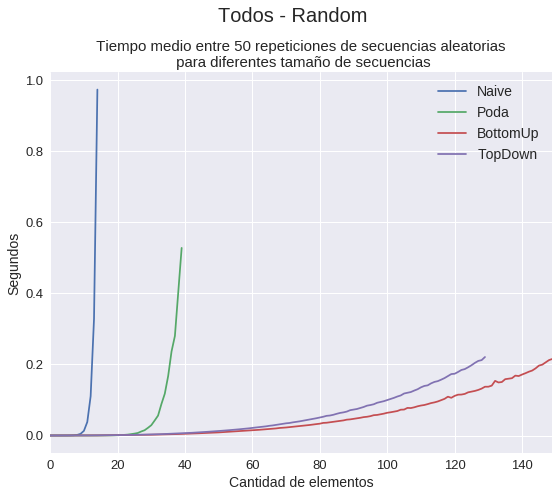
\includegraphics[width=0.75\textwidth]{informe/img/experimentos/todos-random.png} \\
} 

Era esperable que el algoritmo con \textit{poda} sea mucho mas eficiente que el algoritmo \textit{naive}, pero veamos mas de cerca que pasa con los de programación dinámica: \\

% ESTE PODRIA SACARSE PARA AHORRAR LUGAR ... 
% {\centering
%   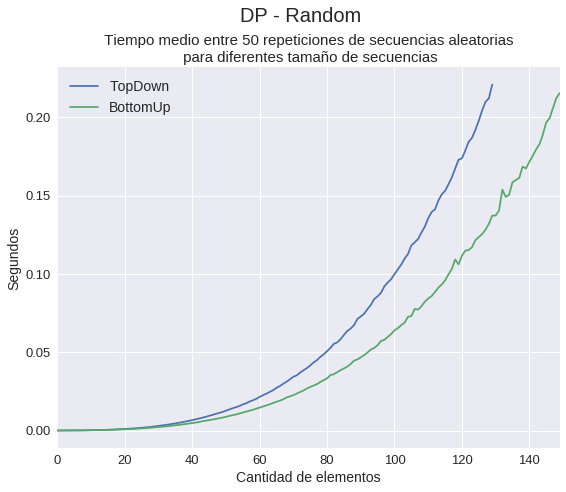
\includegraphics[width=0.75\textwidth]{informe/img/experimentos/dp-random.png} \\
% }

Para instancias de tamaño $\leq 40$ \textit{BottomUp} y \textit{TopDown} se comportan de manera muy similar, pero para tamaños mas grandes las curvas comienzan a separarse. En el análisis teórico, tanto \textit{TopDown} como \textit{BottomUp} tenían la misma complejidad. Lo que podemos deducir de estas mediciones es que \textit{TopDown} tiene una constante oculta mas elevada. Esto es razonable ya que en esta técnica se realizan llamados recursivos y en \textit{BottomUp} no. 

\subsection{Elementos iguales}

En una secuencia donde todos los elementos son iguales, como máximo pueden pintarse un elemento de rojo y otro de azul, pero no más que esto ya que no es posible encontrar secuencias \textit{estrictamente} crecientes o decrecientes. Que sean todos iguales es un buen caso, ya que en rasgos generales las técnicas que revisan la validez de la secuencia a medida que la construyen solo podrían ''entrar'' en la rama donde los elementos no se pintan. \\

El algoritmo de \textit{backtracking naive} tiene tiempos tan malos que no permiten ver con claridad las diferencias entre las otras técnicas, por lo que el gráfico está en \textbf{escala logarítmica} en $y$.\\

En el gráfico podemos ver cómo el \textit{backtracking con poda} es el que produce los resultados mas eficientes. Esto es razonable si consideramos la observación del primer párrafo, y si tenemos en cuenta que los algoritmos de \textit{programación dinámica} siempre crean una matriz de tres dimensiones de tamaño $n^3$, sin importar el contenido de la secuencia. \\

% {\centering
%   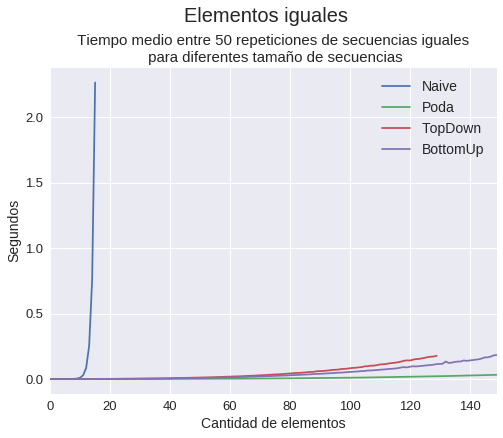
\includegraphics[width=0.75\textwidth]{informe/img/experimentos/todos-iguales.png} \\
% }

{\centering
  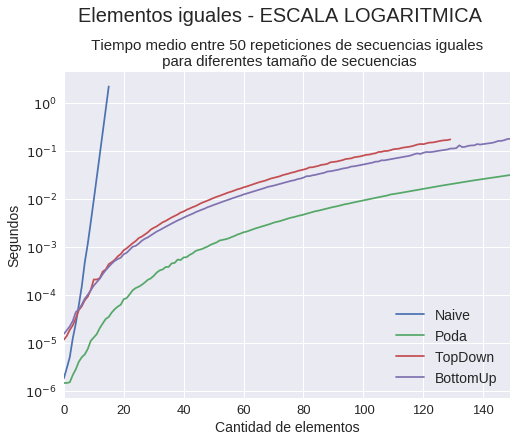
\includegraphics[width=0.75\textwidth]{informe/img/experimentos/todos-iguales-logaritmica.png} \\
}

\subsection{Elementos crecientes}

En una secuencia donde los elementos son \textit{estrictamente crecientes} la solución óptima puede conseguirse pintando todos los elementos del mismo color, obteniendo el mínimo sin pintar en 0. \\

El algoritmo \textit{naive} de backtracking sigue produciendo los peores resultados, ya que siempre revisa todas las combinaciones posibles. Al ser tiempos tan malos, no permiten ver las diferencias con las demás técnicas. Es por esto que el gráfico lo muestro en \textbf{escala logarítmica} en eje $y$.\\

Los algoritmos que usan \textit{programación dinámica} siguen necesitando $O(n^3)$ tiempo para crear la matriz donde van a guardarse los datos, y como en los casos anteriores, \textit{BottomUp} es mas rápido que \textit{TopDown}. \\

Lo interesante lo vemos con el algoritmo \textit{backtracking con poda}, que puede apreciarse que es mucho mas eficiente que todos los demas. (Notar que es aproximadamente el doble de rápido que en los casos donde la secuencia esta formada por números iguales) \\

Esto se debe a que al ser creciente, las ramas con color azul se eliminan rápidamente, y a que una vez encontrado el mínimo valor (el cero) ya no se entrará por los casos donde no se pinta algún elemento. \\

{\centering
  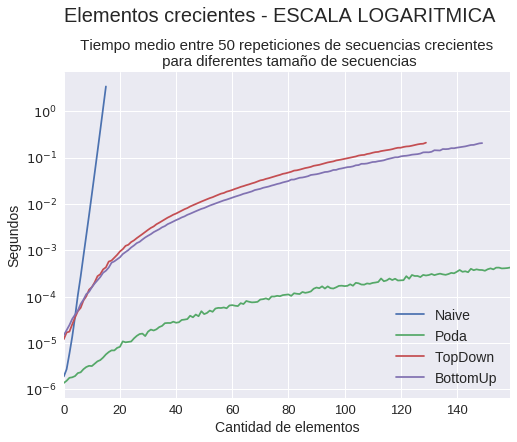
\includegraphics[width=0.75\textwidth]{informe/img/experimentos/todos-creciente-logaritmica.png} \\
}

% NO SE SI NECESARIA
\subsection{Conclusión}

De las técnicas usadas para resolver el problema, en el \textbf{caso general} las soluciones con \textit{programación dinámica} son exponencialemte mejores. \\

Pudimos ver que en \textbf{algunos casos particulares}, por ejemplo cuando la secuencia está formada por los mismos elementos o cuando es creciente (o decreciente), el algoritmo de \textit{backtracking con poda} es el mas eficiente.  \\

Otra gran ventaja de las soluciones \textit{dinámicas}, es que el caso general puede resolverse para tamaños de \textbf{cientos} de elementos, mientras que el algoritmo de \textit{backtracking con poda} es inusable para $n > 60$.  \\

El algoritmo de \textit{backtracking naive} no es bueno en \textbf{ningún} caso, y para $n > 20$ es imposible de utilizar. \\